% !TeX root = ../libro.tex
% !TeX encoding = utf8



\setchapterpreamble[c][0.75\linewidth]{%
	\sffamily
    
    En esta sección se expondrá el desarrollo de los cuatro mejores modelos de la competición llevada a cabo en el año 2017 por la plataforma PhysioNet en la que se usó la misma base de datos la cual se está empleando. También se detallaran tres modelos que se avalan en la literatura por presentar buenos resultados en los problemas para los que fueron planteados. Por último y más importante, se expondrán tres modelos desarrollados propiamente para este problema.
  

	\par\bigskip
}

\chapter{Desarrollo de los modelos}\label{ch:desarrollo}

\section{Modelos Ganadores de la Competición}
        

        Todos los modelos ganadores usan un paradigma común que funciona en dos partes. En la primera se extraen un conjunto de características sobre el problema y en la segunda parte, se aplica clasificación sobre dicho conjunto, lo único que varía son los métodos de extracción y clasificación. Esta forma tiene un ligero problema y es que para la extracción de características los autores requieren de cierto conocimiento previo sobre el campo en cuestión, en este caso ha sido posible, pero de manera general no siempre va a ocurrir. Otro inconveniente es la poca transportabilidad de estos modelos frente a otros problemas. Esto es debido a que los modelos son particularmente diseñados para un problema muy concreto, luego si los intentamos extrapolar a otros ámbitos, posiblemente fallen. 
        
    \subsection{Clasificador binario en cascada}
       
             El artículo de este modelo se puede encontrar en \cite{datta2017identifying}. Los autores consideraron una serie de 209 características que podían ser útiles a la hora de clasificar. Para ello la agruparon en un total de siete conjuntos: Características enfocadas en ECGs con ruido, en particulares de ciertas patologías, en estadísticas, en frecuencias, sobre el ritmo cardiaco, sobre la morfología del ECG y por último en características utilizadas en trabajos anteriores. \\
             
             Tras extraer las características se aplica un clasificador binario en cascada en dos fases. En la primera, el clasificador es entrenado con el objetivo de distinguir entre ECGs normales o con otras patologías y ECGs con fibrilación auricular o ruidosos, es decir, junta la clases N y O por un lado y por otro las clases FA y R para clasificarlas. En la segunda fase se consideran dos nuevos clasificadores. Uno de ellos clasifica las clases N y O que previamente se habían juntado y el otro las clases FA y R. \\ 
             
    \subsection{Encase}
        
            Este modelo es un clasificador diseñado por ensemble, esto es, un clasificador construido a partir de un conjunto de clasificadores resumiendo la salida para obtener una única predicción. Este método lo que primero hace es descomponer el ECG en un conjunto de datos más reducido. Tras hacer esta separación se calcula la onda más informativa del electrocardiograma, conocida como \textit{centerwave} y después se aplican varios extractores de características para terminar aplicando el ensemble de clasificadores. \\
            
            En el funcionamiento que hemos explicado hemos obviado una gran cantidad de detalles, este modelo es el más complejo de todos y se puede consultar en \cite{hong2017encase}
            
          
        
    \subsection{Marco de Interpretación Abductivo}
        
            Este método parte de la creación de un marco de razonamiento completo que trabaja con señales temporales médicas. Destacamos que este método fue diseñado por investigadores españoles de la universidad de Santiago de Compostela, \cite{teijeiro2017arrhythmia}. Primeramente, se extrae la información sobre la morfología del ECG por medio del razonador abducctivo y se construyen 79 característias globales del electrocardiograma. Después se aplica un algoritmo de \textit{gradient boosing} combinado con una red neuronal recurrente y un voto por ponderación para realizar la clasificación. \\
        
    \subsection{Clasificador basado en Random Forest}
            
            Este algoritmo también aplica la extracción de características de manera manual y después se aplica un clasificador simple para ordenarlas por orden de importancia a la hora de clasificar señales. Según se explica en \cite{zabihi2017detection} se generaron un total de 491 características para después aplicar un \textit{random forest} y seleccionar la 150 más informativas. Tras ello, se diseña un clasificador para realizar las predicciones sobre el conjunto reducido. \\
    
    
\newpage 
\section{Modelos en la Literatura}

    Vamos a exponer un conjunto de arquitecturas encontradas en la literatura que presentan buenos resultados según los autores. Comentamos previamente que las arquitecturas son fijas en el sentido de que no se ha realizado ninguna prueba para escoger los hiperparámetros de los modelos ya que de hacerse así se estaría contaminando la arquitectura tomada de la literatura. \\
    
    Existen otros parámetros como el algoritmo de optimización, el tamaño del batch, tamaño de ventana etcétera que si convendrían escogerlos de manera experimental. Se realizó pues un proceso experimental probando distintos hiperparámetros, sin embargo, la mayoría presentaban los mismos resultados, puesto que como más adelante se comentará, estos modelos dan lugar a un gran sobreajuste y la elección de los hiperparámetros no influye apenas. Por este motivo, se omitirá la parte experimental. 
    
    
    \begin{table}[H]
        \caption{Hiperparámetros usados en los modelos. Para OhShuLih y GaoJunLi el tamaño de ventana es igual a 3000 mientras que para ChenChen es la propia arquitectura la que exige un tamaño de ventana algo mayor, por este motivo se ha tomado 5000. El optimizador usado ha sido \textit{Adam} con el learning rate que presenta por defecto. Adam es un optimizador muy recomendable en la literatura y de ahí su elección. El tamaño del batch no puede ser muy grande ya que origina un fallo en la memoria de los servidores GPU, pero tampoco puede ser demasiado pequeño por temas de eficiencia, de este modo, se ha considerado como óptimo el seleccionado. El número de épocas empleadas han sido 300 para que la red se entrene lo suficiente, aunque a veces no se lleguen a completarlas todas gracias a la técnicas de Early Stopping con valor de la paciencia 50. Por otra parte, se ha reducido el tamaño de la serie porque si se deja toda la longitud, los resultados empeoran. En cuanto a la generación de datos, los resultados empeoran si se activa y por este motivo se ha desactivado. }
        \begin{center}
        \begin{tabular}{|l|l|}
        \hline
        \multicolumn{1}{|c|}{\textbf{Parámetros}} & \multicolumn{1}{l|}{Valores} \\ \hline
        \textbf{Batch size} & 128 \\ \hline
        \textbf{Epochs} & 300 \\ \hline
        \textbf{Patiente} & 50 \\ \hline
        \textbf{n\_split} & 5 \\ \hline
        \textbf{reduce} & True \\ \hline
        \textbf{generator} & False \\ \hline
        \textbf{windows\_size} & 3000-5000 \\ \hline
        \textbf{lr} & 0,001 \\ \hline
        \textbf{opt} & Adam \\ \hline
        \end{tabular}
        \end{center}
        \label{fig:hiper_lit}
    \end{table}
    
    \subsection{OhShuLi}
    
        Presentamos un modelo presente en la literatura \cite{ohshuli}, al cual nos referiremos con el nombre del autor, OhShuLih. En el artículo se comenta los buenos resultados que ofrece esta arquitectura, la cual consta de 6 capas convolucionales en las que se incluyen capas de max pooling. Estas capas se encargan de extraer características espaciales de las señales y la última capa de LSTM se encarga de capturar la dependencia en la dinámica temporal de la serie. Finalmente se incluyen tres capas totalmente conectadas. En la imagen \ref{fig:ohshuli_1} podemos ver la arquitectura de esta red en el artículo en donde fue propuesta. \\
        
        \begin{figure}[htpb]
            \centering
            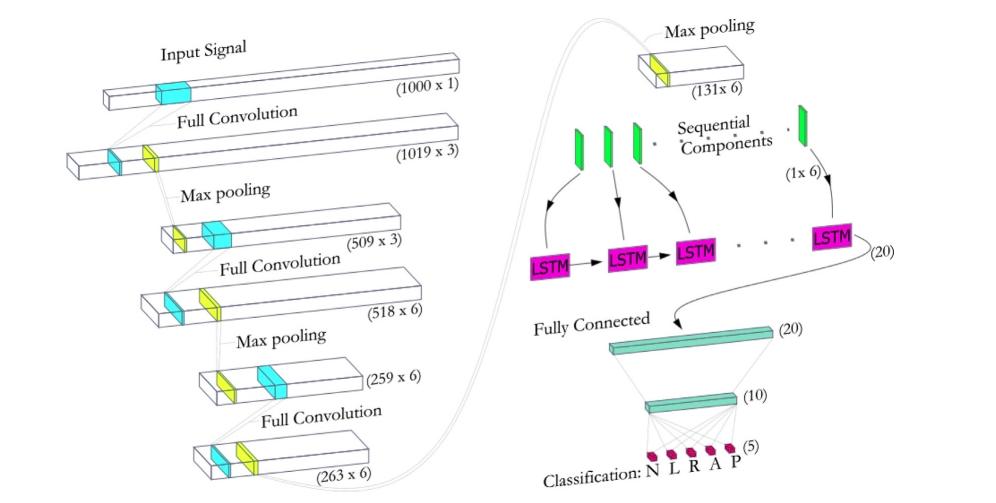
\includegraphics[height=20cm,width=17cm,keepaspectratio]{img/ohshuli1.png}
            \caption{Una ilustración de la arquitectura OhShuLi}
            \label{fig:ohshuli_1}
        \end{figure}
        
        \begin{figure}[htpb]
            \centering
            \includegraphics[width=\textwidth,height=\textheight,keepaspectratio]{img/ohshuli_plot.png}
            \caption{Esquema de la arquitectura OhShuLi. Parámetros entrenables $3254$. Esta arquitetura consta de 3 capas convolucionales de 3, 6 y 6 filtros con un tamaño de kernel de 20,10 y 5 respectivamente. La celda LSTM consta de 20 unidades y las capas capas totalmente conectadas constan de 20,10 y 4 neuronas respectivamente.}
            \label{fig:ohshuli_2}
        \end{figure}
        
        
        
        
    \subsection{ChenChen}
    
        Esta arquitectura la podemos encontrar en \cite{chenchen}. En este artículo se comenta brevemente por encima las ventajas y desventajas de los métodos existentes en cuanto a diagnósticos clínicos, tras lo cual se propone esta arquitectura (Fig \ref{fig:chenchen1},\ref{fig:chenchen2}) con el objetivo de analizar y reconocer seis clases de segmentos de ECG, incluyendo N, AFIB, B, P, AFL y ABR. El artículo justifica el empleo de capas CNN+LSTM explicando que las capas convolucionales se encaran de la extracción automática de características, y el empleo de LSTM se usa en el intervalo entre dos picos R adyacentes para mejorar el rendimiento de identificación. La combinación de CNN más LSTM contribuyen a la extración de información espacial y temporal de las señales y a la mejora de la capacidad de abstracción del modelo. Este artículo empleó como bases de datos: \textit{MIT-BITH}, \textit{AFDB} y \textit{NSRDB}. \\
    
            \begin{figure}[htpb]
                \centering
                \includegraphics[width=\textwidth,height=\textheight,keepaspectratio]{img/chenchen2.png}
                \caption{Esquema de la arquitectura ChenChen. Parámetros entrenables: $91751$}
                \label{fig:chenchen2}
            \end{figure}
            
            \begin{figure}[htpb]
                \centering
                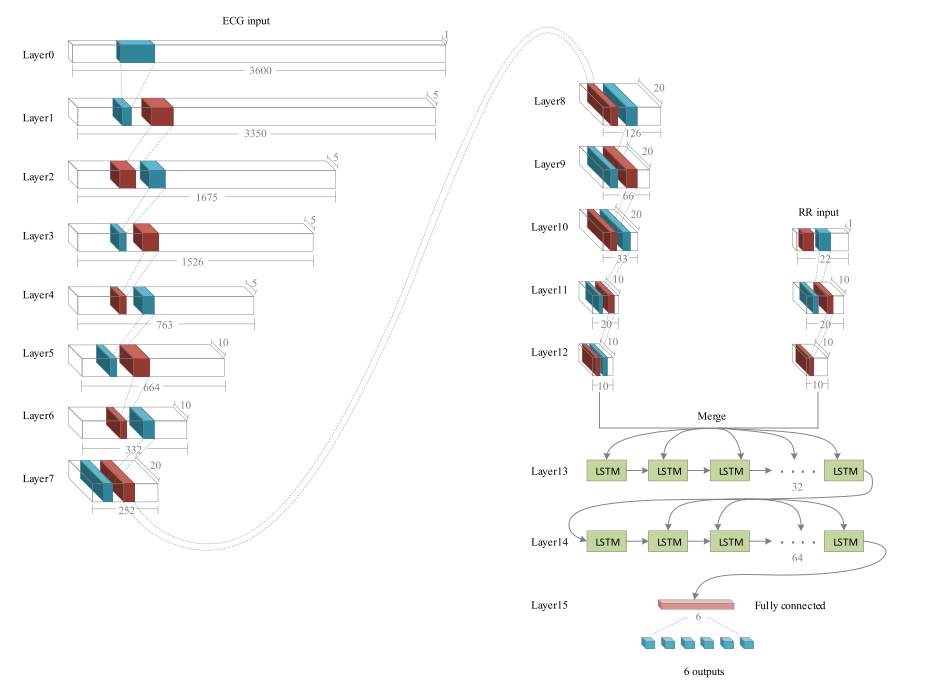
\includegraphics[height=17cm,width=15cm,keepaspectratio]{img/chenchen1.png}
                \caption{Una ilustración de la arquitectura ChenChen. Se han aplicado 6 capas de convolución con 251,150,100,81,61 y 14 filtros y con un tamaño del kernel de 5,5,10,20,20,10 respectivamente. Las capas LSTM tienen 32 y 64 unidades cada una respectivamente.}
                \label{fig:chenchen1}
            \end{figure}
        
    
    
        
    \subsection{GaoJunLi}
    
    Este modelo fue propuesto en \cite{GaoJunLi} y es específico para conjunto de datos con desbalanceo de clase, de hecho el nombre del artículo es \textit{An Effective LSTM Recurrent Network to Detect Arrhythmia on Imbalanced ECG Dataset}. El artículo argumenta que el desequilibrio del conjunto de datos del ECG es un reto adicional para clasificar con precisión los latidos del ECG. Hay dos problemas en el proceso de entrenamiento: (1) la baja eficiencia del entrenamiento, porque los latidos normales del ECG que ocupan una gran proporción del conjunto de datos son propensos a los efectos negativos, y (2) la degeneración del modelo cuando un latido normal del ECG sobrecarga el entrenamiento. Tras lo cual comenta que algunos investigadores han intentado abordar el desequilibrio en los datos de los latidos del ECG a la hora de diagnosticar la arritmia siendo este artículo uno de esos intentos. \\
    
    
    Dado que los datos de los latidos del ECG existen en una categoría muy desequilibrada, se propone un modelo eficaz de red de recurrencia de memoria a corto plazo (LSTM) con pérdida focal (FL). Para ello, la red LSTM puede desentrañar las características de sincronización en las señales complejas de ECG, mientras que la FL se utiliza para resolver el desequilibrio de categorías mediante la reducción de la ponderación de los ejemplos de ECG normales fácilmente identificados. Las ventajas de la red propuesta se han verificado en la base de datos de arritmias MIT-BIH. Los resultados experimentales muestran que la red LSTM con FL logró una solución fiable al problema de los conjuntos de datos desequilibrados en la clasificación de latidos de ECG y no fue sensible a la calidad de las señales de ECG. El método propuesto puede utilizarse en escenarios de telemedicina para ayudar a los cardiólogos a diagnosticar con mayor precisión y objetividad las señales de ECG. En la imagen \ref{fig:gaojunlin} podemos ver la arquitectura de esta red.  \\
    
    
    
        \begin{figure}[htpb]
                \centering
                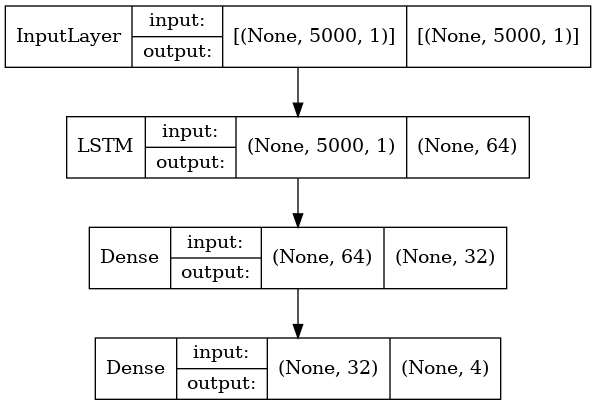
\includegraphics[width=\textwidth,height=\textheight,keepaspectratio]{img/GaoJunLin.png}
                \caption{Esquema de la arquitectura GaoJunLin. Total de parámetros entrenables: $19108$ }
                \label{fig:gaojunlin}
        \end{figure}
            
\newpage
\section{Modelos propios}
    
        Tres propuestas distintas de modelos propios se han desarrollado, el primer modelo basado puramente en convoluciones unidimensionales lo llamaremos CNN, el segundo modelos además de convoluciones unidimensionales tiene unidades LSTM y por ello lo denotaremos con el nombre LSTM y finalmente el tercer y último tipo de modelo lo llamaremos GRU por estar formado por unidades GRU además de convoluciones unidimensionales. \\
        
        La elección de los parámetros tales como el número de filtros de las capas convolucionales, el tamaño del kernel, así como el número de unidades GRU y LSTM y algunos otros parámetos como el nivel de \textit{drop out} o el tipo de padding fueron escogidos en base a un proceso experimental expuesto en la siguiente sección. Otros hiperparámetros, como los de la tabla \ref{fig:hiper_lit} los hemos fijado de antemano.\\
        
        La arquitectura de los modelos (escogidas según el proceso de experimentación que se expondrá en la sección siguiente) las podemos apreciar en las tablas \ref{table:arquitectura modelo cnn}, \ref{table:arquitectura modelo lstm} y \ref{table:arquitectura modelo gru}. En las cuales podemos ver el tipo de capa, el tamaño de la salida y el número de unidades que componen las capas de convolución (unidades entendidas como filtros) y las capas densas (unidades entendidas como neuronas). \\
        
    \subsection{CNN}
        Los hiperparámetros tuneados en este modelo han sido el porcentage de \textit{drop out}, el número de filtros, el tamaño del kernel y el tipo de padding. El \textit{drop out} es un aspecto clave que contribuye a la disminución de sobreajuste. El número de filtros convolucionales y el tamaño del kernel son los dos aspectos más importantes de las redes convolucionales, por lo que un estudio previo sobre los parámetros oportunos es de obligado cumplimiento. El tipo de \textit{padding} es algo que afeta en menor medida, aún así se ha decidido estudiar qué influencia tiene. En la tabla \ref{table:arquitectura modelo cnn} podemos ver la arquitectura. \\
        
        \begin{table}[htpb]
            \caption{Arquitectura Modelo CNN}
            \begin{center}
            %\resizebox{\columnwidth}{!}{%
            \begin{tabular}{|l|l|r|}
            \hline
            \textbf{Layer} & \textbf{Output Shape} & \multicolumn{1}{l|}{\textbf{Units}} \\ \hline
            Conv1D + ReLu + MaxPooling & (None,3000,256) & 128 \\ \hline
            MaxPooling + Drop Out & (None,1500,256) & 0 \\ \hline
            Conv1D + ReLu & (None,1500,256) & 128 \\ \hline
            MaxPooling + Drop Out & (None,750,256) & 0 \\ \hline
            Conv1D + ReLu & (None,750,128) & 64 \\ \hline
            MaxPooling + Drop Out & (None,375,128) & 0 \\ \hline
            Conv1D + ReLu & (None,375,85) & 42 \\ \hline
            MaxPooling + Drop Out & (None,187,85) & 0 \\ \hline
            Conv1D + ReLu & (None,187,64) & 32 \\ \hline
            MaxPooling + Drop Out & (None,93,64) & 0 \\ \hline
            Conv1D + ReLu & (None,93,51) & 25 \\ \hline
            MaxPooling + Drop Out & (None,46,51) & 0 \\ \hline
            Conv1D + ReLu & (None,46,42) & 21 \\ \hline
            MaxPooling + Drop Out & (None,23,256) & 0 \\ \hline
            Global Average Pooling & (None,42) & 0 \\ \hline
            Dense + Relu + Drop Out & (None,128) & 128 \\ \hline
            Dense + Relu + Drop Out & (None,64) & 64 \\ \hline
            Dense + Relu + Drop Out & None,32) & 32 \\ \hline
            Dense + Softmax & (None,4) & 0 \\ \hline
            \textbf{Total Parámetros} & 1288656 & \\ \hline
            \end{tabular}
            %}
            \end{center}
            \label{table:arquitectura modelo cnn}
            \end{table}
    
    \subsection{LSTM}
        Los parámetros usados para este modelo han sido las unidades de LSTM, las neuronas de las últimas capas densas y el tipo de padding. El número de unidades en la capa LSTM es un aspecto fundamental y que no debe de ser pasado por alto. El número de unidades en las últimas capas densas también es importante por ese motivo también ha sido estudiado. Notamos que el número de hiperparámetros aquí es mucho menor que el anterior, esto se debe en parte a que este tipo de modelos gastan gran cantidad de tiempo en ejecución dificultando la realización de un estudio más detallado. El valor de \textit{drop out} se ha fijado a $0,4$. En la tabla \ref{table:arquitectura modelo lstm} podemos ver la arquitectura. \\
        
    
        \begin{table}[htpb]
            \caption{Arquitectura Modelo LSTM}
            \begin{center}
            %\resizebox{\columnwidth}{!}{%
            \begin{tabular}{|l|l|r|}
            \hline
            \textbf{Layer} & \textbf{Output Shape} & \multicolumn{1}{l|}{\textbf{Units}} \\ \hline
            Input & (None,3000,1) & 0 \\ \hline
            Zero Padding & (None,3008,1) & 0 \\ \hline
            Conv1D & (None,3004,128) & 128 \\ \hline
            Max Pooling & (None,1502,128) & 0 \\ \hline
            Zero Padding & (None,1510,128) & 0 \\ \hline
            Conv1D & (None,1506,64) & 64 \\ \hline
            Max Pooling & (None,753,64) & 0 \\ \hline
            Zero Padding & (None,761,64) & 0 \\ \hline
            Conv1D & (None,757,32) & 32 \\ \hline
            Max Pooling & (None,378,32) & 0 \\ \hline
            Zero Padding & (None,386,32) & 0 \\ \hline
            Conv1D & (None,382,8) & 8 \\ \hline
            Max Pooling & (None,191,8) & 0 \\ \hline
            LSTM + Drop Out & (None,16) & 16 \\ \hline
            Dense + ReLu + Drop Out & (None,32) & 32 \\ \hline
            Dense + Softmax & (None,4) & 4 \\ \hline
            \textbf{Total Parámetros} & 55396 & \\ \hline
            \end{tabular}
            %}
            \end{center}
            \label{table:arquitectura modelo lstm}
            \end{table}
            
    \subsection{GRU}
    
        Los parámetros usados para este modelo han sido el número de unidades GRU y el número de neuronas en las capas densas. Estos dos hiperparámetros son los más importantes del modelo y los de obligatorio estudio. El resto de hiperparámetros se han fijado a un valor y no se han tenido en cuenta para el estudio por los motivos expuestos en el modelo anterior. El valor de \textit{drop out} se ha fijado a $0,4$. En la tabla \ref{table:arquitectura modelo gru} podemos ver la arquitectura. \\
        
    
        
            \begin{table}[htpb]
            \caption{Arquitectura Modelo GRU}
            \begin{center}
            %\resizebox{\columnwidth}{!}{%
            \begin{tabular}{|l|l|r|}
            \hline
            \textbf{Layer} & \textbf{Output Shape} & \multicolumn{1}{l|}{\textbf{Units}} \\ \hline
            Input & (None,3000,1) & 0 \\ \hline
            Zero Padding & (None,3008,1) & 0 \\ \hline
            Conv1D & (None,3004,128) & 128 \\ \hline
            MaxPooling & (None,1502,128) & 0 \\ \hline
            Zero Padding & (None,1510,128) & 0 \\ \hline
            Conv1D & (None,1506,64) & 64 \\ \hline
            Max Pooling & (None,753,64) & 0 \\ \hline
            Zero Padding & (None,761,64) & 0 \\ \hline
            Conv1D & (None,757,32) & 32 \\ \hline
            Max Pooling & (None,378,32) & 0 \\ \hline
            Zero Padding & (None,386,32) & 0 \\ \hline
            Conv1D & (None,382,8) & 8 \\ \hline
            Max Pooling & (None,191,8) & 0 \\ \hline
            GRU + Drop Out & (None,25) & 25 \\ \hline
            Dense + ReLu + Drop Out & (None,32) & 32 \\ \hline
            Dense + Softmax & (None,4) & 4 \\ \hline
            \textbf{Total Parámetros} & 56709 & \\ \hline
            \end{tabular}
            %}
            \end{center}
            \label{table:arquitectura modelo gru}
            \end{table}


%        \newpage
%        \begin{figure}[H]
%             \centering
%             \begin{subfigure}[b]{0.3\textwidth}
%             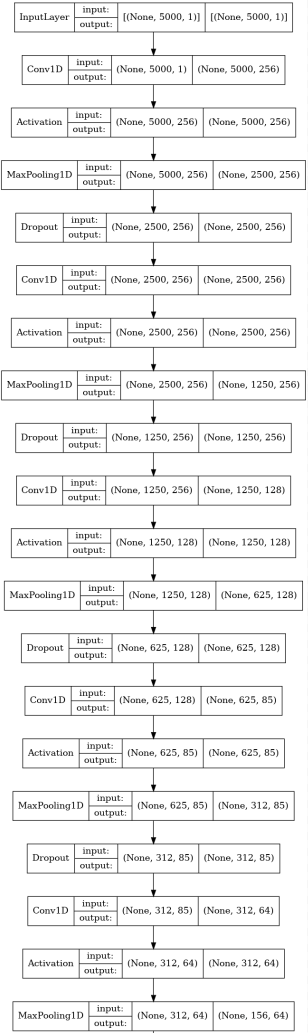
\includegraphics[height=\textheight,keepaspectratio]{img/arq_mod_1_1.png}
%             \end{subfigure}
%             \hfill
%             \begin{subfigure}[b]{0.3\textwidth}
%             \includegraphics[height=\textheight,keepaspectratio]{img/arq_modelo_1_2.png}
%             \end{subfigure}
%             \caption{Esquema de la arquitectura CNN.}
%             \label{fig:arquitectura modelo cnn}
%         \end{figure}
%
%       
%        \begin{figure}[H]
%                \centering
%                \includegraphics[width=\textwidth,height=\textheight,keepaspectratio]{img/modelo2.png}
%                \caption{Esquema de la arquitectura LSTM.}
%               \label{fig:arquitectura modelo lstm}
%        \end{figure} 
%        
%        \begin{figure}[H]
%                \centering
%                \includegraphics[width=\textwidth,height=\textheight,keepaspectratio]{img/modelo2.png}
%                \caption{Esquema de la arquitectura GRU.}
%                \label{fig:arquitectura modelo gru}
%        \end{figure} 
        
        
       
    
    

    
\endinput